%versi 3 (22-07-2020)
\chapter{Landasan Teori}
\label{chap:teori}

\section{Teknologi pembuatan \web}
\label{sec:web} 
 
Menurut KBBI \web adalah sistem untuk mengunduh, mengakses, atau memanipulasi informasi yang ada di dalam komputer yang dihubungkan melalui internet. Seiring dengan perkembangan waktu \web dibangun dengan menggunakan berbagai macam teknologi.
Teknologi-teknologi yang dipakai untuk membuat \web dibagi ke dalam dua bagian yaitu teknologi untuk membuat \textit{front-end} dan teknologi untuk membuat \textit{back-end}. \textit{Web} yang sudah jadi kemudian diukur performanya. Performa dari sebuah web diukur menggunakan matriks penilaian. Penilaian performa ini didasarkan pada pengalaman pengguna \web yang akan dinilai. Diterjemahkan dari Zigisova dalam bukunya matriks penilaian yang digunakan adalah \textit{Core Web Vitals} dimana matriks ini memiliki tiga komponen penilaian utama yang mencakup penilaian performa saat memuat konten, penilaian tingkat interaktif, dan penilaian stabilitas visual.~\cite{WebAlmanac.2024.Performance}. Matriks-matirks penilaian ini yang akan dianalisis

\section{\textit{Structure Query Language}}
\label{sec:sql}
\textit{Structure Query Language} atau yang biasa disebut SQL merupakan bahasa pemrograman yang bertujuan untuk memanipulasi atau mengubah basis data. Ben Forta dalam bukunya menjelaskan bahwa bahasa ini didesain untuk mengerjakan sebuah perintah dengan tepat dan benar agar proses pembuatan atau pengambilan data berjalan lebih efisien~\cite{ben}. Data disimpan dalam bentuk tabel ke dalam basis data, untuk mengakses data tersebut SQL menyediakan beberapa sintaks yang bisa dipakai. Sintaks yang dapat dipakai adalah sebagai berikut:
\begin{itemize}
    \item \verb|SELECT| dan \verb|FROM| merupakan sintaks yang berguna untuk memilih bagian data yang dibutuhkan dari tabel tertentu.
    \item \verb|WHERE| adalah sintaks yang berguna untuk memberikan kondisi tertentu dalam memilih data.
    \item \verb|GROUP BY| adalah sintaks yang berguna untuk mengelompokan data berdasarkan kelas tertentu yang terdapat dalam data.
    \item \verb|JOIN| adalah sintaks yang berguna untuk menggabungkan dua buah tabel. Penggabungan data ini bisa dibagi kedalam beberapa cara yaitu \textit{inner join, outer join, right join, self join}.
\end{itemize}
sintaks-sintaks tersebut merupakan sebagian kecil dari sintaks yang dimiliki oleh bahasa SQL.

\section{Statistika}~\cite{han:22:datmin}
\label{sec:stat}

Statistika adalah ilmu yang mempelajari tentang eksplorasi, analisis, implementasi, dan pengumpulan data. Statistika memiliki beberap properti untuk melihat \textit{Central Tendency} dari data. \textit{Central Tendency} adalah pusat kumpulan sebuah data. Properti yang dapat digunakan untuk melihat pusat kumpulan data adalah sebagai berikut:
\begin{itemize}
    \item \textit{Mean} atau rata-rata adalah properti untuk mengukur distibusi nilai dari sebuah data. Persamaan~\ref{eq:mean} digunakan untuk mencari nilai rata-rata dari sebuah data. $N$ merupakan jumlah data yang sedang diamati sedangkan nilai $x_N$ merupakan nilai-nilai yang akan dijumlahkan mulai dari $x_1$ hingga $x_N$.

    \begin{equation}
    \label{eq:mean}
        \bar{x} = \frac{x_1+x_2+x_3+...+x_N}{N}
    \end{equation}

     \item \textit{Median} merupakan nilai tengah dari data yang sedang diamati. Nilai \textit{median} dapat dicari dengan cara mengasumsikan bahwa data telah terurut, nilai $N$ nmerupakan jumlah data kemudian jika $N$ memiliki nilai yang ganjil maka letak nilai \textit{median} nya terpadapat pada posisi $\frac{N+1}{2}$, sedangkan jika nilai $N$ nya genap maka nilai \textit{median} nya terletak pada posisi $\frac{N}{2}$.

     \item \textit{Mode} atau modus adalah nilai yang kemunculanya paling banyak pada sebuah data.
\end{itemize}

Properti lain yang dapat digunakan selain \textit{Central Tendency} adalah pengukuran distribusi dan sebaran data, beberapa properti yang dapat digunakan adalah sebagai berikut:
\begin{itemize}
    \item \textit{Max} merupakan nilai paling besar dari sebuah data.
    \item \textit{Min} merupakan nilai paling kecil dari sebuah data.
    \item \textit{Range} merupakan perbedaan dari nilai paling besar dengan nilai paling kecil
    \item  \textit{Variance} dan Standar Deviasi adalah metode untuk mengukur sebaran data. \textit{Variance} didapatkan dengan cara mengkuadratkan perbedaan setiap titik pada data dengan rata-ratanya, sedangkan standar deviasi merupakan akar dari \textit{variance}. \textit{Variance} cenderung menghasilkan nilai yang lebih besar dari nilai-nilai yang terdapat pada data asli karena merupakan hasil kuadtrat, sedangkan standar deviasi cenderung menghasilkan nilai yang hampir sama dengan nilai-nilai yang terdapat pada data asli. Standar deviasi dapat dicari dengan menggunakan Rumus~\ref{eq:sd}, dimana nilai $N$ adalah jumlah data, nilai $X_i$ adalah nilai ke-i dari atribut $X$, dan $\bar{X}$ merupakan nilai rata-rata dari atribut $X$.
    \begin{equation}
    \label{eq:sd}
        \sigma = \sqrt{
        \begin{pmatrix}
            \frac{1}{N} \sum_{i=1}^NX_i^2
        \end{pmatrix}
        -\bar{X}^2}
    \end{equation}
    Semakin besar nilai standar deviasinya maka dapat dikatakan bahwa data semakin tersebar dari nilai rata-ratanya, sebaliknya semakin kecil nilai standar deviasinya maka dapat dikatakan bahwa data semakin dekat sebaranya dari nilai rata-ratanya.
\end{itemize}

\section{Visualisasi Data}
\label{sec:visdat}

\subsection{Bar Plot}
\label{subsec:barplot}

\begin{figure}[h]
    \centering
    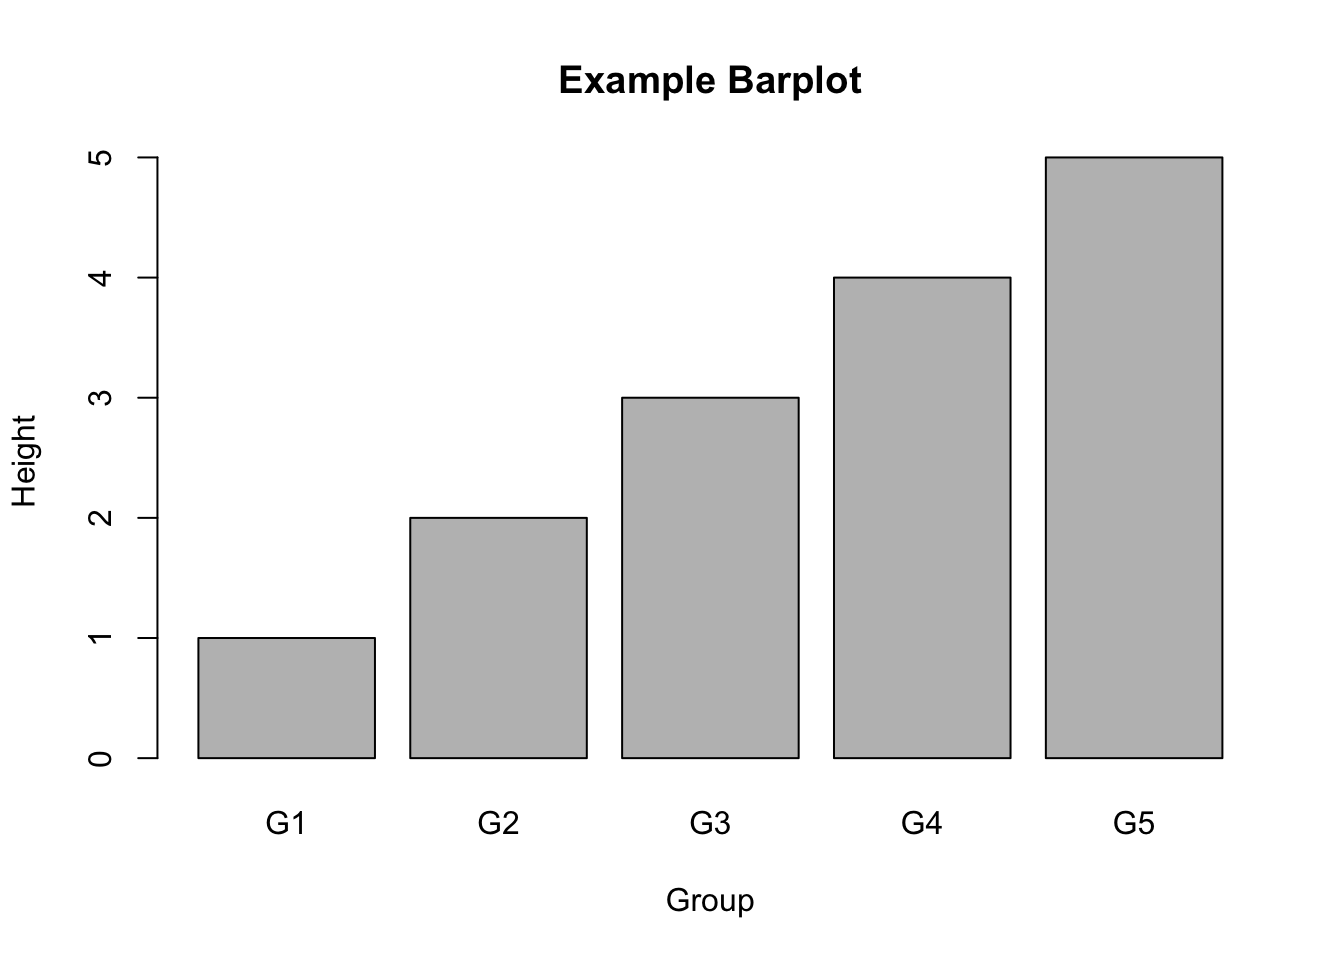
\includegraphics[width=0.4\linewidth]{Gambar/contoh barplot.png}
    \caption{Contoh visualisasi dari tinggi beberapa grup dengan menggunakan \textit{bar plot}}
    \label{fig:contoh barplot}
\end{figure}

\textit{Bar plot} merupakan teknik visualisasi data yang menggunakan batang vertikal atau horizontal untuk menunjukkan nilai-nilai dari data. Visualisasi ini berguna untuk menunjukkan pengukuran statistik sebuah data secara terpisah. \textit{Bar Plot} memiliki elemen utama yaitu sumbu \textit{x} dan sumbu \textit{y}. Gambar~\ref{fig:contoh barplot}~\cite{Phillips} merupakan contoh penggunaan \textit{bar plot} untuk memvisualisasikan data di mana pada contoh ini sumbu \textit{x} nya menunjukkan grup yang dimiliki data sedangkan sumbu \textit{y} nya menunjukkan tinggi dari masing-masing grup.